% !TEX encoding = UTF-8
% !TEX TS-program = pdflatex
% !TEX root = ../Appunti.tex

\section{Introduzione}

In seguito si considera un modello di \textit{gas perfetto} per illustrare alcune delle affermazioni generali fatte.

\begin{defn}[Gas perfetto]
	Un \textit{gas perfetto} è un insieme di particelle (o, generalizzando, strutture elementari) \textit{non interagenti}.
\end{defn}

Per rendere il sistema \textit{non integrabile}, e quindi \textit{ergodico}, si deve però assumere che ci sia qualche modo per far scambiare impulso fra le particelle, e quindi farle interagire. Si può pensare ad un interazione mediata dalle pareti della scatola che contiene il gas.

\paragraph{Osservabili macroscopiche} A livello microscopico il sistema è quindi caratterizzato dall'Hamiltoniano di singola particella, e non c'è altro da aggiungere. Si vuole però caratterizzare il sistema nel suo insieme attraverso delle \textit{osservabili macroscopiche} e trovare le relazioni fra esse: si vuole trovare \textit{l'equazione di stato} del sistema complessivo.

Si vuole quindi indagare a livello microscopico l'origine di concetti macroscopici quali: \textit{entropia}, \textit{irreversibilità} e \textit{equilibrio}.

\subsection{Principi della Meccanica Statistica}
Per colmare il salto che separa la descrizione \textit{microscopica} dalle proprietà \textit{macroscopiche} del sistema la Meccanica Statistica di equilibrio pone essenzialmente due principi:

\begin{description}
	\item[Perdita di memoria:] all'equilibrio, che si suppone sempre raggiunto da un sistema dopo un tempo sufficientemente lungo (rispetto alle scale temporali delle interazioni microscopiche), il \textit{macrostato} del sistema è indipendente dalle condizioni iniziali.
	\item[Equiprobabilità a priori:] all'equilibrio ogni possibile \textit{microstato} è equiprobabile. La disponibilità di un data microstato dipende dai vincoli che deve soddisfare il sistema (es.: conservazione dell'energia).
\end{description}

\subsubsection{Equilibrio}

Si è parlato di \textit{equilibrio}, senza specificare cosa si intenda per esso. Non è una questione banale, ma a questo livello se ne può dare una definizione approssimativa.

\begin{defn}[Equilibrio]
	\label{def:eq}
	Si dice che un sistema macroscopico è all'\textit{equilibrio} quando tutte le osservabili macroscopiche sono \textit{stazionarie}, cioè non evolvono nel tempo.
\end{defn}

La \cref{def:eq} è approssimativa in quanto si considereranno in seguito trasformazioni fra stati di equilibrio.
\`E però una buona definizione se si specifica che la scala temporale su cui va valutata la stazionarietà è \textit{mesoscopica}: per tempo \textit{microscopici} il sistema evolve secondo la dinamica data dalle singole interazioni, mentre a livello \textit{macroscopico} l'evoluzione è data dalla trasformazione considerata.

Infatti per mantenere la condizione di equilibrio la scala microscopica e quella macroscopica sono separate da diversi ordini di grandezza, per cui è possibile la verifica della stazionarietà delle osservabili su scale intermedie, che vanno però considerate come nettamente distinte dalle altre (si può pensare a tre stati diversi, analogamente all'elettronica digitale in confronto alla natura analogica dei segnali).

\paragraph{Sulla natura dei principi fisici} \`E importante tenere presente che le due assunzioni fatte sono \textit{principi}, quindi non necessariamente verificati per ogni sistema fisico, ma sperimentalmente veri per un buon numero di sistemi e assunti per tutti gli altri.

A differenza di altri principi, che connettono l'astrazione teorica al mondo fisico, per natura stessa della meccanica statistica questi connettono due branche della teoria, quella microscopica e quella macroscopica, per cui è possibile che queste assunzioni siano false a livello formale per alcune classi di sistemi. Questo è il caso dei sistemi \textit{integrabili} (e quindi \textit{non ergodici}) in meccanica classica, ed è il caso di quasi tutti i sistemi quantistici (in cui la situazione è molto più sottile).

\'E sufficiente però considerare che questi sistemi sono pochi nel caso classico, mentre nel caso quantistico il problema si aggira in un altro modo, per cui i principi considerati consentono la descrizione di una classe enorme di sistemi (la quasi totalità).

\subsection{Entropia}
\label{sec:entro}

Si supponga che il sistema abbia $\Gamma$ possibili microstati, con $\Gamma \equiv \Gamma(E,N,V)$, cioè una funzione del volume, dell'energia e del numero totale dei componenti (d'ora in avanti \textit{particelle}) del sistema.

\begin{defn}[Entropia, microscopica]
	L'\textit{entropia} di un sistema è definita in base alle proprietà microscopiche di un sistema come:
	\begin{equation*}
	S = k \log\Gamma
	\end{equation*}
\end{defn}

In questo modo anche l'entropia è una funzione di volume, energia e numero di particelle del sistema $S \equiv S(E,N,V)$.

Invertendo l'entropia come funzione dell'energia si ottiene $E(S,N,V)$, e da questa espressione si possono studiare le variazioni dell'energia totale.

\begin{equation*}
	\dd E = \left(\frac{\partial E}{\partial S}\right)_{N,V} \dd S + \left(\frac{\partial E}{\partial V}\right)_{S,N} \dd V + \left(\frac{\partial E}{\partial N}\right)_{S,V} \dd N
\end{equation*}

\begin{note}[Invertibilità di $S(E,N,V)$]
	\'E sempre possibile invertire l'entropia in funzione dell'energia a $V$ e $N$ fissati, infatti se non c'è un limite superiore per l'energia di singola particella il numero di microstati sarà una funzione crescente dell'energia, e quindi anche l'entropia.
\end{note}

\paragraph{Osservabili intensive} Le osservabili estensive caratteristiche di un sistema macroscopico $E, N, V$ sono state definite in modo naturale a partire dalle caratteristiche microscopiche.

A questo punto si possono definire le osservabili intensive dalle variazioni dell'energia, distinguendo le varie sorgenti.

\begin{defn}[Osservabili Intensive]
	\label{def:ossint}
	Si definisce \textit{temperatura:}
	\begin{equation*}
	T = \left(\frac{\partial E}{\partial S}\right)_{N,V}
	\end{equation*}
	
	Si definisce \textit{pressione:}
	\begin{equation*}
	P = - \left(\frac{\partial E}{\partial V}\right)_{S,N}
	\end{equation*}
	
	Si definisce \textit{potenziale chimico:}
	\begin{equation*}
	\mu = \left(\frac{\partial E}{\partial N}\right)_{S,V}
	\end{equation*}
\end{defn}

Le definizioni che si sono date sono del tutto \textit{formali}, a priori senza alcun senso fisico alle spalle. Si esamina quindi una di queste (la temperatura) per capire la corrispondenza della definizione a un concetto fisico.

\paragraph{Temperatura} Il concetto fisico di temperatura è dato dal \textit{principio zero} della termodinamica: essa è una caratteristica del sistema che ne descrive l'equilibrio termico rispetto ad altri sistemi. La temperatura è quindi un numero reale:
\begin{itemize}
	\item condiviso per sistemi fra loro all'equilibrio;
	\item per sistemi non in equilibrio indica il verso in cui fluisce il calore.
\end{itemize}

Quando due sistemi, con numero di microstati $\Gamma_1$ e $\Gamma_2$, sono separati, il numero di microstati totale sarà $\Gamma_1\Gamma_2$.
Quando i sistemi sono posti in contatto, a $V$ e $N$ fissati per ciascuno, tutto ciò che può succedere macroscopicamente è che una parte dell'energia di uno fluisca nell'altro, e per la monotonicità dell'entropia quindi se aumenta $S_1$ allora diminuirà $S_2$ e viceversa.

Se i sistemi sono all'equilibrio l'entropia totale è allora in un massimo, altrimenti aumenterebbe tramite scambio di energia. Inoltre anche l'energia totale è conservata, per cui:

\begin{align*}
&\begin{rcases*}
\delta(E_1 + E_2) = 0 \\
\delta E_i = T_i \delta S_i
\end{rcases*}
\implies T_1 \delta S_1 + T_2 \delta S_2 = 0 \\
&\delta(S_1 + S_2) = 0
\end{align*}

\noindent Da cui si ottiene facilmente $T_1 = T_2$.

Si può verificare anche l'affermazione sul verso del flusso di energia (calore): sia $T_1 < T_2$, l'energia è sempre conservata, inoltre si considera che l'entropia totale può solo aumentare:

\begin{align*}
&\begin{rcases*}
\delta(E_1 + E_2) = 0 \\
\delta E_i = T_i \delta S_i
\end{rcases*}
\implies T_1 \delta S_1 + T_2 \delta S_2 = 0 \implies \implies \delta S_1 = - \frac{T_2}{T_1} \delta S_2\\
& \delta(S_1 + S_2) \geq 0 \implies \delta S_1 \geq - \delta S_2
\end{align*}

Da cui si ottiene:

\begin{equation*}
- \frac{T_2}{T_1} \delta S_2 \geq - \delta S_2 \implies (1 - \frac{T_2}{T_1}) \delta S_2 \geq 0 \implies \delta S_2 \leq 0
\end{equation*}

E per la monotonicità dell'entropia si ha anche $\delta E_2 \leq 0$, che corrisponde a quanto atteso.

\paragraph{Equazione di stato} A questo punto si è in grado di calcolare, astrattamente, l'\textit{l'equazione di stato}, eliminando l'entropia dalle due equazioni:

\begin{align*}
	&T(S,V,N) = \left(\frac{\partial E}{\partial S}\right)_{N,V} \\
	&P(S,V,N) = - \left(\frac{\partial E}{\partial V}\right)_{S,N}
\end{align*}

\subsection{Precisazioni teoriche sui fondamenti}
\label{sec:teorpipterm}
Anche se le temperatura di due sistemi è la stessa l'operazione di metterli a contatto non è senza conseguenze: si perde traccia dell'energia esatta di ognuno dei due sistemi, mantenendo l'informazione su quella totale.

Per cui si pongono due questioni:
\begin{itemize}
	\item quanta incertezza viene introdotta?
	\item negli argomenti usati precedentemente nello studio della temperatura, funziona tutto bene anche avendo perso traccia delle singole energie nel contatto termico?
\end{itemize}

La risposta alla prima domanda è: sostanzialmente poca, ed è per questo che la meccanica statistica funziona bene (si veda la \cref{sec:fluct}, per una trattazione più estesa).

La risposta alla seconda domanda è che non ci serve sapere quantitativamente l'energia, ma che è sufficiente sapere che il sistema è isolato e la sua energia è fissata.
\newline

C'è un punto ancora più sottile: oltre all'incertezza termodinamica sull'energia, se consentiamo le transizioni fra microstati a livello quantistico non siamo in uno stato stazionario, ma in stati con tempo di vita finito, e quindi vi è un'incertezza del tutto quantistica sulla loro energia.

Comunque se il numero di particelle è abbastanza grande questa incertezza non è rilevante: $\Gamma \sim 10^N$, per cui se anche l'errore sul conteggio degli stati fosse dell'ordine di $ N $ l'errore sul logaritmo (cioè sull'entropia) diventa irrisorio per grandi $ N $.

\paragraph{Descrizione canonica} Si può però rinunciare alla descrizione \textit{microcanonica} (energia fissata, vedi \cref{sec:statmech}) e decidere di considerare un piccolo sottosistema di un grande sistema isolato: per esso non sarà fissata l'energia, ma la temperatura, attraverso il contatto col resto del sistema che fungerà da \textit{bagno termico}.

L'energia del sistema quindi sarà libera di fluttuare, ma la descrizione si sposterà sulla \textit{densità di stati}, che non è soggetta a incertezza quantistica.

\begin{note}[Legge di dispersione]
	La \textit{densità di stati} tipicamente è determinata dal seguente procedimento:
	\begin{itemize}
		\item si assume che sia piatta sullo spazio delle fasi accessibile;
		\item si trasforma in una funzione dell'energia, una volta nota l'energia come funzione degli impulsi e delle poszioni.
	\end{itemize}
	Quest'ultima è a volte nota come \textit{legge di dispersione}.
\end{note}

\subparagraph{Fluttuazioni} \`E importante distinguere fra due tipi di fluttuazioni:
\begin{description}
	\item[fluttuazioni microscopiche:] si è detto che un sistema in equilibrio esplora tutti i microstati accessibili \textit{ergodicamente}, ma questo tipo di fluttuazioni fra microstati non sono fluttuazioni dell'equilibrio: l'equilibrio ha origine proprio da una media su queste transizioni;
	\item[fluttuazioni macroscopiche:] quando si è introdotto l'approccio \textit{canonico} si è inserita la possibilità che l'energia non fosse fissata, ma fluttuasse; queste fluttuazioni sono di tipo macroscopico, perché al livello microscopico descritto prima tanto il microcanonico quanto il canonico fluttuano.
\end{description}

% quest'ultima parte sulle fluttuazioni va rivista graficamente e dal punto di vista dell'italiano.

\section{Termodinamica}
\label{sec:termod}


\subsection{I principi della termodinamica}
La \textit{termodinamica} è fondamentalmente un sistema logico basato su quattro assiomi.

\paragraph{Principio zero} Il principio zero è stato già citato e discusso nella \cref{sec:teorpipterm}, esso caratterizza la relazione di equilibrio termico fra sistemi. Si riporta lo stesso un enunciato conciso:

\begin{defn}[Principio zero della termodinamica]
	La relazione di equilibrio termico è transitivi, quindi è una relazione di equivalenza.
	
	Più esplicitamente: se A è in equilibrio con B e con C, allora B è in equilibrio con C.
\end{defn}

\begin{note}
	C'è da fare attenzione anche in questo caso all'applicabilità fisica di questo principio: la verifica dell'equilbrio termico è effettuata mediante contatto termico, per cui per stabilire che due corpi non sono in equilibrio è necessario veder fluire calore.
	
	Se il calore che fluisce non è poco due corpi non in equilibrio potrebbero diventarlo. Cioè: la verifica dell'equilibrio fra due corpi può alterare la situazione iniziale, anzi, in generale \textbf{deve} farlo.
	
	Per aggirare questo problema ci si può servire di corpi sufficientemente piccoli di test (detti \textit{termometri}) che possono mediare il processo di verifica della situazione di equilibrio senza alterare apprezzabilmente lo stato dei corpi da testare, ed è in questo senso che va inteso il principio zero.
\end{note}

\paragraph{Primo principio} Il primo principio asserisce la \textit{conservazione dell'energia}: esso, macroscopicamente, corrisponde all'istituzione stessa di una quantità, detta energia, che si conservi in sistemi isolati.

\begin{defn}[Primo principio della termodinamica]
	L'energia è una quantità conservata per sistemi isolati.
	
	Più esplicitamente: se l'energia interna a un sottosistema del sistema isolato globale (da qui in poi detto \textit{universo}) non è conservata, essa è stata scambiata con altre parti dell'universo. Lo scambio di energia può assumere due forme: lavoro meccanico o calore.
	
	\begin{equation*}
		\dd E = \dd Q + \dd W
	\end{equation*}
	
	$Q$ è il calore assorbito dal sottosistema, mentre $W$ è il lavoro fatto sul sottosistema.
\end{defn}

\noindent Si noti che il lavoro meccanico corrisponde ad un trasporto di energia \textit{macroscopico}, mentre il calore è essenzialmente un trasporto di energia \textit{microscopico}. Questa è la principale differenza tra i due.

Per il \textit{gas perfetto} si può legare il lavoro alla variazione delle osservabili macroscopiche:

\begin{equation*}
\dd W = \mathcal{F} \dd x = \frac{\mathcal{F}}{A} (A\dd x) = - P \dd V
\end{equation*}

\noindent In generale è possibile identificare il lavoro, nell'ambito della meccanica lagrangiana, fermandosi alla prima uguaglianza e considerando come $\dd x$ gli spostamenti generalizzati e com $ \mathcal{F} $ le forze generalizzate corrispondenti (bisognerà inoltre sommare su tutti i possibili contributi).
\newline

Si ottiene quindi che:
\begin{equation*}
	\left(\frac{\partial E}{\partial V}\right)_Q = - P
\end{equation*}

\noindent Che può essere confrontato con la definizione data nella \cref{sec:entro}.

Questo è legato al fatto che una trasformazione \textit{isoentropica} avviene senza scambio di calore, infatti variando in modo sufficientemente lento il volume per il \textit{teorema adiabatico} i microstati cambieranno, ma ci sarà una corrispondenza uno a uno fra vecchi e nuovi, quindi il loro numero è fissato.

Queste ultime affermazioni in realtà sono tutte nell'ottica della meccanica statistica, perché a livello termodinamico l'entropia è definita nell'ambito del \textit{secondo principio}, che non è stato ancora esposto.

\paragraph{Secondo principio} Il secondo principio è enunciato nel modo più termodinamicamente corretto nelle forme di \textit{Kelvin} e di \textit{Clausius}, ben note e reperibili. Esse consentono la dimostrazione del teorema di \textit{Carnot}, e conseguentemente di quello di \textit{Clausius}, che consente di definire l'entropia.

Si sceglie allora di assumere noto il teorema di \textit{Clausius}, definendo l'entropia, e servendosi di essa per enunciare il secondo principio, ma deve essere noto che questo non è realmente possibile in termodinamica, in quanto il secondo principio è logicamente precedente alla definizione stessa di entropia.

\begin{defn}[Entropia]
	La variazione di entropia fra uno stato A e uno stato B è:
	\begin{equation*}
	\Delta S = \int_{A \rightarrow B} \frac{\dd Q}{T}
	\end{equation*}
	dove l'integrazione è effettuata su un cammino costituito da una trasformazione \textit{reversibile}.
	
	L'entropia è quindi definita così a meno di una costante, che fissa il valore dell'entropia per un certo stato.
\end{defn}

\noindent E dunque:

\begin{defn}[Secondo principio della termodinamica]
	L'entropia di un sistema isolato fuori equilibrio tende ad aumentare.
\end{defn}

\noindent Gli stati di equilibrio sono quindi caratterizzati come massimi dell'entropia.

\paragraph{Terzo principio} Il terzo principio si colloca ai margini della termodinamica, e più che farne parte ne specifica i limiti. Infatti esso afferma che:

\begin{defn}[Terzo principio della termodinamica]
	L'entropia a temperatura nulla (zero assoluto) è nulla.
\end{defn}

\noindent che in modo equivalente può essere inteso come: \textit{la temperatura nulla non è raggiungibile da processi termodinamici.}

\subsection{Grandezze termodinamiche}
\label{sec:thermquant}

Vi sono quattro variabili termodinamiche principali, non indipendenti:

\begin{equation*}
\begin{matrix}
S	&	V \\
T	&	P \\
\end{matrix}
\end{equation*}

\noindent Organizzate nel modo seguente:
\begin{itemize}
	\item la prima riga sono estensive;
	\item la seconda riga intensive;
	\item le variabili appartenenti alla stessa colonna sono coniugate.
\end{itemize}

\noindent Le variabili coniugate compaiono a coppie nell'espressione dell'energia. Ogni variabile termodinamica può essere espressa come funzione della variabile coniugata e di una delle altre due (si verifica a partire dalle espressioni date nella \cref{def:ossint}).

Perciò è sempre possibile scegliere una coppia di variabili, non coniugate, come \textit{indipendenti}, le altre due saranno quindi \textit{dipendenti} e ottenibili come funzioni delle prime.
\newline

Le variabili termodinamiche scelte come \textit{dipendenti} possono essere ricavate da un singolo \textit{potenziale termodinamico}, se le variabili indipendenti scelte sono le variabili \textit{proprie} del potenziale.

I potenziali termodinamici sono ottenuti come opportune trasformate di Legendre dell'energia, si passa quindi ad illustrarli.

\paragraph{Energia E} Le sue variabili proprie sono $S$ e $V$. L'espressione del suo differenziale è:

\begin{equation*}
\dd E = T \dd S - P \dd V
\end{equation*}

\paragraph{Energia libera F} Le sue variabili proprie sono $T$ e $V$. La sua espressione in funzione dell'energia $E$ è:

\begin{equation*}
F = E - T S
\end{equation*}

E dunque l'espressione del suo differenziale è:

\begin{equation*}
\dd F = - S \dd T - P \dd V
\end{equation*}

\begin{note}
	Le variabili proprie dell'energia libera sono particolarmente comode (il motivo è per lo più che non contengono l'entropia), per cui essa è decisamente utile ai fini del calcolo dell'equazione di stato, cioè $ P(V,T) $ (un altro motivo è che si esprime in modo semplice in termini della \textit{funzione di partizione}, vedi \cref{sec:statmech}).
\end{note}

\paragraph{Energia libera di Gibbs G }Le sue variabili proprie sono $T$ e $P$. La sua espressione in funzione dell'energia $E$ è:

\begin{equation*}
G = E - T S + P V
\end{equation*}

E dunque l'espressione del suo differenziale è:

\begin{equation*}
\dd G = - S \dd T + V \dd P
\end{equation*}

\begin{note}
	Anche questo potenziale ha una sua utilità specifica: esso è espresso in funzione delle variabili \textit{intensive}, questo lo rende particolarmente per caratterizzare alcune situazioni (es: \textit{transizioni di fase}).
\end{note}


\paragraph{Entalpia H}Le sue variabili proprie sono $S$ e $P$. La sua espressione in funzione dell'energia $E$ è:

\begin{equation*}
H = E + P V
\end{equation*}

E dunque l'espressione del suo differenziale è:

\begin{equation*}
\dd H = T \dd S + V \dd P
\end{equation*}

Si nota che l'entalpia ha una proprietà per cui in inglese è chiamata anche \textit{heat function}, ed è:

\begin{equation*}
\dd H)_P = T \dd S)_P = \dd Q)_p
\end{equation*}

\subsubsection{Relazioni di Maxwell}
Applicando il \textit{teorema di Schwarz} (di cui supponiamo sempre verificate le ipotesi, lontano da punti critici) si ha la commutazione delle derivate seconde, e applicando questo risultato ai vari potenziali termodinamici si ottengono le cosiddette \textit{relazioni di Maxwell}.

Si riporta solo il caso dell'energia libera a titolo di esempio:

\begin{equation*}
\left(\frac{\partial P}{\partial T}\right)_V = \frac{\partial}{\partial T} \left(- \left(\frac{\partial F}{\partial V}\right)_T\right)_V = \frac{\partial}{\partial V} \left(- \left(\frac{\partial F}{\partial T}\right)_V\right)_T = \left(\frac{\partial S}{\partial V}\right)_T
\end{equation*}

\`E noto un diagramma che riassume le proprietà dei potenziali termodinamici, cioè le variabili proprie e le relazioni di Maxwell, ed è considerato un utile strumento mnemonico (\cref{fig:maxrel}).

\begin{figure}[t]
	\centering
	\input{MaxRel.pdf_tex}
	\caption{Diagramma illustrativo delle relazioni fra potenziali termodinamici (noto anche come \textit{diagramma di koenig} )}
	\label{fig:maxrel}
\end{figure}

\subsubsection{Numero di particelle}
Fino ad adesso si è considerato costante il numero di particelle, ma in base alla scelta che si fa del sottosistema anche esso può essere variabile: non è necessario che un sottosistema sia identificato dalla scelta di alcune particelle, che in generale è impossibile da effettuare (vedi \cref{secidpart}), ma potrebbe essere descritto da altre proprietà (es: il volume che occupa, un certo insieme di stati, \dots).

Perciò, coerentemente con la \cref{def:ossint}, si può scrivere:

\begin{equation*}
\dd E = T \dd S - P \dd V + \mu \dd N
\end{equation*}

\noindent Da questa inoltre risultano le espressioni degli altri potenziali termodinamici, ottenute differenziando le opportune trasformate di Legendre.

\begin{note}
	Un'importante osservazione è che le variazioni dei potenziali termodinamici rispetto a qualunque nuova osservabile, tenendo costanti le variabili proprie, sono tutte uguali, infatti:
	
	\begin{equation*}
	\mu \delta N = (\delta E)_{S, V} = (\delta F)_{T,V} = (\delta G)_{T,P} = (\delta H)_{S,P}
	\end{equation*}
\end{note}

Inoltre si noti che $E$ è una grandezza estensiva, le cui variabili proprie sono anch'esse estensive; sfruttando questa proprietà si ha che scalando di una quantià $\lambda$ il sistema\footnote{Si immagini di frazionare in parti il sistema, se il sistema è sufficientemente grande posso coprire tutto $\mathbb{Q}^+$, e passando al limite $\mathbb{R}^+$.}:

\begin{align*}
& \dd (\lambda E) = T \dd (\lambda S) - P \dd (\lambda V) + \mu \dd (\lambda N) \implies\\ 
& \qquad \implies E \dd \lambda + \lambda \dd E  = T (S \dd \lambda + \lambda \dd S) - P (V \dd \lambda + \lambda \dd V) + \mu (N\dd \lambda + \lambda \dd N)
\end{align*}

Raccogliendo $\lambda$ e $\dd lambda$, e considerando che poiché $\lambda$ è arbitrario le due identità risultanti devono essere soddisfatte separatamente, si ottiene l'equazione di Eulero:

\begin{equation*}
E = TS - PV + \mu N
\end{equation*}

Da cui si ottiene l'espressione per la variazione del potenziale chimico:

\begin{equation*}
\dd \mu = - \frac{S}{N} \dd T + \frac{V}{N} \dd P
\end{equation*}

L'equazione di Eulero per l'energia implica che anche gli altri potenziali termodinamici possano avere una forma simile. In particolare:

\begin{equation*}
G = \mu N
\end{equation*}

\paragraph{Gran Potenziale $\Omega$} Si può definire un ulteriore potenziale termodinamico, invertendo le nuove variabili $N \rightarrow \mu$. Le sue variabili proprie sono $T$, $V$ e $\mu$. La sua espressione in funzione dell'energia $E$ è:

\begin{equation*}
\Omega = F - \mu N = E - TS - \mu N
\end{equation*}

E dunque l'espressione del suo differenziale è:

\begin{equation*}
\dd \Omega = - S \dd T - P \dd V - N \dd \mu
\end{equation*}

Dall'equazione di Eulero si ricava:

\begin{equation*}
\Omega = - P V
\end{equation*}

\subsection{Variabili Magnetiche}
Lo studio del magnetismo in termodinamica è frequente, e la definizione di variabili magnetiche non è affatto dissimile dall'introduzione di pressione e volume per il gas perfetto come forza e spostamento \textit{generalizzati}.

Si nota solo che il ruolo di forza generalizzata in questo ambito è svolto dal campo magnetico $ H $, mentre lo spostamento generalizzato è $ \dd (M V) $ dove $M$ è la magnetizzazione del mezzo e $V$ è ancora il volume.

\subsection{Principio variazionale}
Il principio variazionale fondamentale in termodinamica è quello fissato dal \textit{secondo principio}: l'entropia per uno stato di equilibrio è massima.

Questo si riflette in una serie di principi variazionali ausiliari, dettati dalla possibilità di raggiungere l'equilibrio tenendo costanti alcune delle variabili termodinamiche.

\begin{align*}
	T, V, N = cost. \qquad \implies \qquad F = \text{minimum}\\
	T, P, N = cost. \qquad \implies \qquad G = \text{minimum}\\
	T, V, \mu = cost. \qquad \implies \qquad \Omega = \text{minimum}\\
\end{align*}

Si posson ottenere considerando il sottosistema che fluttua alla ricerca dell'equilibrio e il bagno termico, il cui stato di equilibrio non è influenzato dalle fluttuazioni del sottosistema. Perciò si ha:

\begin{equation*}
\begin{rcases*}
\begin{rcases*}
\dd E' = T \dd S' - \dd W'\\
\delta (E + E') = 0
\end{rcases*} \dd E + T \dd S' - \dd W' = 0\\
\delta (S + S') \geq 0
\end{rcases*}
\delta E \leq T \delta S + p \delta V
\end{equation*}

Dall'ultima espressione si ottiene facilmente l'enunciato per $F$, ponendo $\delta V = 0$ e $T \delta S = \delta (T S)$. Analogamente si può fare per gli altri due casi.

\subsection{Derivate termodinamiche}

Si è visto nella \cref{sec:thermquant} come le variabili termodinamiche possano essere ottenute come derivate prime dei potenziali termodinamici, che costituisce la prima definizione data di alcune di esse (\cref{def:ossint}).

Si consideri d'ora in avanti i potenziali termodinamici come le quantità termodinamiche \textit{massimamente integrate}, le altre grandezze termodinamiche saranno caratterizzate dall'essere ottenute a un qualche ordine di derivazione da esse.

Perciò, se le variabili stesse costituiscono il \textit{primo ordine di derivazione}, si prenderà in esame adesso il \textit{secondo ordine di derivazione}. Si è già parlato di esso nella \cref{sec:thermquant}, a proposito delle \textit{relazioni di Maxwell}; in quell'ambito si sono considerate solo le derivate seconde miste, passiamo quindi a considerare le altre.

\begin{defn}[Capacità termica]
	Si definisce \textit{capacità termica a volume costante} la quantità $C_V$:
	\begin{equation*}
	C_V = T \left(\frac{\partial S}{\partial T}\right)_V
	\end{equation*}
	Si definisce \textit{capacità termica a pressione costante} la quantità $C_P$:
	\begin{equation*}
	C_P = T \left(\frac{\partial S}{\partial T}\right)_P
	\end{equation*}
\end{defn}

\noindent La capacità termica quantifica la variazione di temperatura $\delta T$ in base allo scambio di calore $T \delta S$.

Per la capacità termica $C_V$ si nota la relazione:
\begin{equation*}
C_V = \left(\frac{\partial E}{\partial T}\right)_V
\end{equation*}

\noindent è però importante rendersi conto che la temperatura $T$ non è una delle variabili proprie dell'energia.

Per entrambe le capacità termiche si può esprimere però propriamente in funzione dei potenziali termodinamici con le variabili proprie adeguate:

\begin{align*}
C_V = T \left(\frac{\partial^2 F}{\partial T^2}\right)_V\\
C_P = T \left(\frac{\partial^2 G}{\partial T^2}\right)_P
\end{align*}

\noindent che giustifica il fatto che esse siano grandezze del \textit{secondo ordine} (d'ora in poi è omesso che si tratti di derivate).
\newline

Analogamente si possono definire le \textit{compressibilità}:

\begin{defn}[Compressibilità]
	Si definisce \textit{compressibilità isoterma} la quantità $K_T$:
	\begin{equation*}
	K_T = - \frac{1}{V} \left(\frac{\partial V}{\partial P}\right)_T
	\end{equation*}
	Si definisce \textit{compressibilità adiabatica} la quantità $K_S$:
	\begin{equation*}
	K_S = - \frac{1}{V} \left(\frac{\partial V}{\partial P}\right)_S
	\end{equation*}
\end{defn}

Anche in questo caso è possibile esprimere le compressibilità in funzione di opportune derivate seconde:

\begin{align*}
&K_T = - \frac{1}{V} \left(\frac{\partial^2 G}{\partial P^2}\right)_T\\
&K_S = - \frac{1}{V} \left(\frac{\partial^2 H}{\partial P^2}\right)_S = \left[ V \left(\frac{\partial^2 E}{\partial V^2}\right)_S \right]^{-1}
\end{align*}

\paragraph{Relazioni notevoli} Attraverso la definizione dei differenziali delle variabili termodinamiche si possono ottenere delle importanti relazioni fra le quantità appena definite.
Ad esempio, per le capacità termiche:
\begin{align*}
&\begin{rcases*}
\dd S = \left(\frac{\partial S}{\partial P}\right)_T \dd P + \left(\frac{\partial S}{\partial T}\right)_P \dd T\\
\left(\frac{\partial S}{\partial P}\right)_T = - \left(\frac{\partial V}{\partial T}\right)_P
\end{rcases*}
\qquad \frac{C_V}{T} = \left(\frac{\partial S}{\partial T}\right)_V = \left(\frac{\partial S}{\partial P}\right)_T \left(\frac{\partial P}{\partial T}\right)_V + \frac{C_P}{T} \implies\\
&\qquad \qquad \implies \frac{C_P - C_V}{T} = \left(\frac{\partial V}{\partial T}\right)_P \left(\frac{\partial P}{\partial T}\right)_V
\end{align*}

Da cui si ottiene infine, applicando \textit{chain rule}\footnote{\`E necessario notare che la relazione corretta, dimostrabile mediante l'uso di opportuni Jacobiani, è:
\begin{equation*}
	\left(\frac{\partial V}{\partial T}\right)_P \left(\frac{\partial T}{\partial P}\right)_V \left(\frac{\partial P}{\partial V}\right)_T = -1
\end{equation*}
}:

\begin{equation*}
C_P - C_V = T V K_T \left[\left(\frac{\partial P}{\partial T}\right)_V\right]^2 = \frac{T}{V K_T} \left[\left(\frac{\partial V}{\partial T}\right)_P\right]^2
\end{equation*}

\paragraph{Variabili magnetiche} Anche nel caso di variabili magnetiche le quantità definite dalle derivate seconde non miste sono rilevanti, e vengono chiamate \textit{suscettività.}

\begin{defn}[Suscettività]
	Si definisce \textit{suscettività isoterma} la quantità $K_T$:
	\begin{equation*}
	X_T = \left(\frac{\partial M}{\partial H}\right)_T
	\end{equation*}
	Si definisce \textit{suscettività adiabatica} la quantità $K_S$:
	\begin{equation*}
	X_S = \left(\frac{\partial M}{\partial H}\right)_S
	\end{equation*}
\end{defn}

E anche in questo caso si può ottenere una relazione simile a quella per $C_V$ e $C_T$ nel caso delle capacità termiche a magnetizzazione e campo costante, rispettivamente $C_M$ e $C_H$. 

\begin{equation*}
C_H - C_M = \frac{T V}{X_T} \left[\left(\frac{\partial M}{\partial T}\right)_H\right]^2
\end{equation*}

\subsubsection{Funzioni di risposta} Le quantità definite prima caratterizzano la risposta lineare del sistema agli stimoli esterni, per si ha la seguente definizione:

\begin{defn}[Funzioni di risposta]
	Le capacità, compressibilità e suscettività vengono definite collettivamente \textit{funzioni di risposta.}
\end{defn} 

\paragraph{Proprietà} Si mostrano ora alcune proprietà delle funzioni di risposta:
\begin{itemize}
	\item $K_T \geq 0$: si consideri un sistema isolato con $N,T$ e $V$ costanti, si ha quindi che il sistema tende a minimizzare l'energia libera $F$. Si consideri inoltre il sistema diviso in due parti.
	\begin{align*}
	\begin{rcases*}
	\dd V_1 + \dd V_2 = \dd V = 0\\
	\delta F \geq 0
	\end{rcases*}
		 \frac{\partial F}{\partial V_1} = \frac{\partial F_1}{\partial V_1} + \frac{\partial F_2}{\partial V_1} = \frac{\partial F_1}{\partial V_1} - \frac{\partial F_2}{\partial V_2} = 0
	\end{align*}
	dove si è usato solo che $F$ è in un punto stazionario, e si è trovato infine $P_1 = P_2$, che è intuitivo caratterizzi l'equilibrio meccanico (deriva dall'\textit{equilibrio delle forze}).
	
	Il fatto che $F$ sia in un minimo da un informazione ulteriore sulle derivate seconde:
	\begin{equation*}
	 \frac{\partial^2 F}{\partial V_1^2} =  \frac{\partial}{\partial V_1} (P_2 - P_1) =  -\frac{\partial P_1}{\partial V_1} -\frac{\partial P_2}{\partial V_2} \geq 0 \implies \frac{1}{V_1 K_{T_1}} + \frac{1}{V_2 K_{T_2}} \geq 0
	\end{equation*}
	Considerando le due parti del sistema composte dallo stesso numero di particelle, $N_1 = N_2$, si ottiene che, poiché si è dimostrato che la condizione di equilibrio impone che temperatura e pressione siano anch'esse le stesse (e quindi anche i volumi sono uguali per l'equazione di stato), si ha che $K_{T_1} = K_{T_2}$, da cui la tesi.
	\item $C_V \geq 0$: gli argomenti che si usano nella dimostrazione sono simili al caso precedente, per cui si mettono in luce solo le differenze:
	\begin{itemize}
		\item si considera un sistema con isolato, quindi con $E$ e $V$ costanti, anziché $T$ e $V$;
		\item si ha quindi che il principio variazionale da usare è direttamente quello per $S$, anziché la forma per $F$;
		\item si trova che all'equilibrio le temperature sono uguali, anziché le pressioni.
	\end{itemize}
	\item $C_P \geq 0$: si possono sviluppare argomenti analoghi per $C_P$, ma nella sezione precedente si è dimostrata una relazione notevole per la differenza delle capacità termiche, il cui membro di destra era sempre positivo, per cui: $C_P \geq C_V \geq 0$.
\end{itemize}

Si noti che le proprietà mostrate dovevano risultare vere già a livello concettuale, prima della dimostrazione formale:
\begin{description}
	\item[compressibilità] la positività della compressibilità è equivalente ad affermare che all'aumentare della pressione interna il corpo tenda ad espandersi;
	\item[capacità termica] la positività della capacità termica è equivalente ad affermare che ad un aumento di temperatura corrisponde un aumento di energia interna.
\end{description}

L'intuitività del secondo è minata dal fatto che il concetto di temperatura non è affatto intuitivo, ma piuttosto formale; si recupera in parte l'intuizione ricordando che la temperatura è quella quantità che caratterizza il verso del flusso di calore fra due corpi non all'equilibrio. Per cui il segno della capacità termica è stato \textit{scelto} quando si è scelto che il calore fluisse dal corpo a temperatura più alta verso quello a temperatura più bassa.

\subsection{Diagrammi di fase}

\subsubsection{Digressione sul concetto di fase}
La materia che stiamo considerando è composta da particelle, la cui struttura interna è fissata, ma la struttura che assume l'insieme di questi corpi può dipendere fortemente dalle osservabili macroscopiche. La possibilità di distinguere proprio a livello macroscopico queste tipologie di organizzazione determina il concetto di \textit{fase}.

La definizione del concetto di \textit{fase} non è affato banale, per cui si cita quella data dalla \href{http://www.treccani.it/enciclopedia/fase/#chimica-1}{Treccani}:

\begin{defn}[Fase]
	In un sistema eterogeneo si definiscono f. le parti omogenee, di uguale composizione chimica e di uguale stato fisico, separabili meccanicamente. Così, i gas che sono sempre completamente miscibili formano un’unica f.; i liquidi formano più f. quando sono fra loro non completamente miscibili; i solidi possono dare un illimitato numero di fasi. Più in generale, si chiama f. una qualsiasi porzione di un sistema fisico-chimico per la quale siano costanti tutti i parametri che la individuano chimicamente e fisicamente (pressione, temperatura, densità, entropia, costituzione chimica ecc.).
\end{defn}

Questa è una buona definizione a livello enciclopedico, forse un po' povera se confrontata col livello di formalità generale. La cosa importante è chiarire esplicitamente a livello concettuale cosa implica la nozione di fase, per cui si prova a caratterizzarla:

\begin{itemize}
	\item essa è chiaramente riferita ad una porzione estesa di materia, per cui è richiesta una certa coerenza fra le proprietà \textit{mesoscopiche} all'interno della regione spaziale considerata, al punto da poterle considerare uniformi; è importante considerare le proprietà mesoscopiche, perché:
	\begin{itemize}
		\item si vogliono considerare punti spazialmente diversi (le proprietà macroscopiche riguardano l'intero sistema, per cui non possono dipendere dal punto);
		\item non si stanno considerando le proprietà microscopiche, che invece variano drasticamente sulle scale tipiche delle singole particelle (si pensi agli atomi e i campi elettrici).
	\end{itemize}
	\item proprio per l'uniformità richiesta tale nozione implica un certo ordine, un certo tipo di organizzazione (o la sua assenza) che si ripete nei vari punti dello spazio; a posteriori, pensando ai vari tipi di fase noti, è chiaro il senso di questa affermazione. 
\end{itemize}

\subsubsection{Piano $P-T$}

La presenza delle varie fasi è ben visualizzabile nel piano $P-T$. La \cref{fig:phdiagr} illustra il caso tipico di un diagramma delle fasi.

\begin{wrapfigure}{R}{0.5\textwidth}
	\vspace{-30pt}
	\centering
	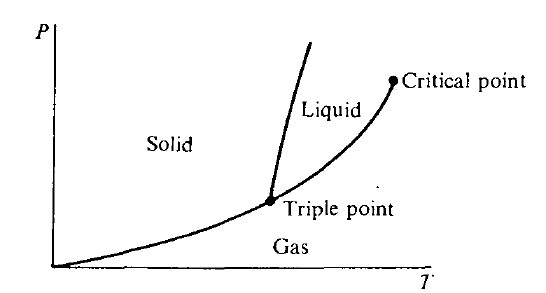
\includegraphics[width=0.5\textwidth]{Immagini/PhaseDiagram.png}
	\caption{}
	\label{fig:phdiagr}
	\vspace{-30pt}
\end{wrapfigure}

Ci sono varie osservazioni da fare:
\begin{itemize}
	\item la più importante è la scelta delle variabili $P-T$, esse sono variabili intensive, e il motivo è chiaro: se la \textit{fase} è caratterizzata dall'uniformità essa non potrà direttamente dipendere da proprietà estensive quali il volume, infatti raddoppiando il sistema (numero di particelle compreso) esso manterrà lo stesso tipo di ordine, sarà solo più grande;
	\item le linee marcate nel diagramma sono note come \textit{linee di coesistenza}, e in quei punti nel sistema sono presenti le due fasi contemporaneamente; essendo oggetti $1$-D sono individuati da una sola variabile, infatti fissata una fra pressione e temperatura l'altra è determinata dalla condizione di coesistenza;
\end{itemize}

\begin{itemize}
	\item il punto di intersezione fra le due linee di coesistenza è detto \textit{punto triplo}, in esso coesistono le tre fasi, ed è individuato da una esatta pressione e temperatura;
	\item la lineaa di coesistenza tra \textit{liquido} e \textit{gas} termina in un punto critico: questo implica che non si può realmente distinguere fra l'uno e l'altro, perché è possibile cambiare fase in modo continuo, aggirando tale punto\footnote{\`E però evidente che se il punto critico è piuttosto distante è abbastanza facile distinguere tra liquido e gas, perché potreste non essere praticamente possibile realizzare un percorso che aggiri il punto critico.}.
\end{itemize}

Si riporta inoltre un altro diagramma, relativo al piano $P-V$:

\begin{figure}[H]
	\centering
	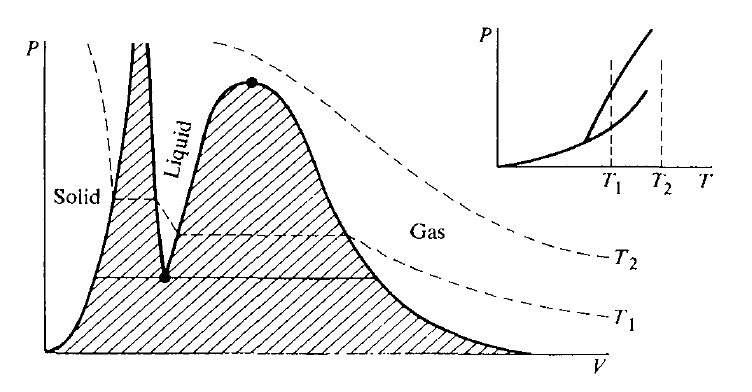
\includegraphics[width=0.7\textwidth]{Immagini/PhasePV.png}
	\caption{}
	\label{fig:phasepv}
\end{figure}

Ciò che si vuole evidenziare di esso è che la \textit{"traiettoria"} delle curve isoterme (tratteggiate in figura) nella regione tratteggiata (regione di coesistenza): esse coincidono con delle isobare, corentemente con quanto descritto a proposito delle curve di coesistenza.
Le variabili $P$ e $T$ non sono quindi sufficienti in questa regione a descrivere il sistema, poiché a $P$ e $T$ fissati sono possibili diversi valori di $V$.

Quello che sta accadendo è che $V$ descrive quanta parte del sistema è in una o in un'altra fase, poiché nella varie fasi cambia il \textit{volume specifico} $V/N$; per cui nella regione ad alto $V$ il sistema sarà prevalentemente nella fase ad alto volume specifico, e viceversa nella regione a basso $V$.

Ci sono altre cose interessanti da notare in questo grafico: la posizione del punto critico e quella del punto triplo, la \textit{separazione} tra solido e liquido, la transizione "diretta" da gas a solido. Si lascia al lettore lo studio di questa proprietà sul diagramma.

\subsubsection{Equazione di Clausius-Clapeyron}

Nella \cref{fig:phdiagr} si può inoltre notare come tutte le curve di coesistenza abbiano derivata sempre positiva. Questa è una proprietà frequente, ma non necessaria.

Il motivo è il seguente, e verrà verificato a posteriori: se l'entropia specifica e il volume specifico crescono in modo concorde da una fase all'altra la pendenza della curva sarà positiva, se discorde sarà negativa.

Intuitivamente ciò che succede è che ad alta temperatura sarà privilegiata la fase più entropica (ha un peso maggiore nell'energia libera di Gibbs) mentre ad alta pressione quella a più alta densità, quindi più basso volume specifico. Se una stessa fase soddisfa entrambi i requisiti allora la pendenza della curva sarà negativa, e la variazione discorde, viceversa nell'altro caso. 
\newline

Per ricavare il risultato precedente si consideri un sistema isolata, costituito da due sottosistemi, che condividono lo stesso volume e lo stesso insieme di particelle, e sono distinti dallo stato: ciascuno rappresenta una diversa fase.

Dalle condizioni di equilibrio ricavate precedentemente si ha $T_1 = T_2$ e $P_1 = P_2$. Un ulteriore condizione si ottiene considerando:
\begin{align*}
\begin{rcases*}
\dd N_1 + \dd N_2 = \dd V = 0\\
\delta F \geq 0
\end{rcases*}
\frac{\partial F}{\partial N_1} = \frac{\partial F_1}{\partial N_1} + \frac{\partial F_2}{\partial N_1} = \frac{\partial F_1}{\partial N_1} - \frac{\partial F_2}{\partial N_2} = 0
\end{align*}

\noindent Perciò $\mu_1 = \mu_2$.

Da questa uguaglianza si può ricavare un'equazione per $P$ e $T$:

\begin{equation*}
\mu_1 (P,T) = \mu_2 (P,T)
\end{equation*}

Per cui si può risolvere per una delle due variabili e ottenere l'equazione esplicita della curva (si noti che se le fasi che coesistono fossero tre ci sarebbe un'altra equazione da soddisfare, cioè l'uguaglianza con $\mu_3$, questo porterebbe ad individuare un unico punto, il punto triplo).

Per ricavarsi l'equazione della curva è quindi necessaria l'espressione esplicita del potenziale chimico in funzione delle due variabili indicate. Questa può essere ricavata da una teoria microscopica delle fasi.

Si può comunque ricavare un utile risultato dalla relazione di Gibbs-Duhem:

\begin{align*}
&\dd \mu_1 = \dd \mu_2 \implies -s_1 \dd T + v_1 \dd P = -s_2 \dd T + v_2 \dd P \implies \\
&\qquad \implies \derivative{ P_0}{T} = \frac{s_2 - s_1}{v_2 - v_1}
\end{align*}

\noindent dove si è usato $s = S/N$ e $v = V/N$, rispettivamente entropia e volume specifici.

In questo ambito si definisce inoltre il \textit{calore latente}:

\begin{defn}[Calore latente]
	\`E una grandezza $\lambda$ delle dimensioni di un'energia (un calore), che caratterizza le transizioni di fase discontinue, cioè quelle in cui è presente una differenza finita di entropia specifica tra le due fasi.
	\begin{equation*}
		\lambda = T(s_2 - s_1) = T \Delta s
	\end{equation*} 
\end{defn}

Alla luce di questa nuova definizione l'equazione di Clausius-Clapeyron è espressa in modo naturale come:

\begin{equation*}
\derivative{ P_0}{T} = \frac{\lambda}{T(v_2 - v_1)}
\end{equation*}

\section{Meccanica Statistica}
\label{sec:statmech}

Il compito della meccanica statistica è principalmente \textit{contare il numero di stati possibili} per un dato macrostato, cioè trovare $\Gamma(E,V,N)$, come indicato nella \cref{sec:entro}.

Da esso infatti sarà possibile trovare l'espressione per l'entropia, e invertendo ques'ultima si avrà l'energia in funzione delle sue variabili proprie, che determina in modo completo la dinamica macroscopica.

In reltà non è conveniente cercare di ottenere $E(S,V,N)$, perché l'entropia non è una variabile così naturale, specie dal punto di vista sperimentale. Si cercherà invece di ottenere la funzione $ F(T,V,N) $, oppure $ \Omega(T,V,\mu) $, le cui variabili proprie risultano molto più intuitive (si ribadisce che l'equazione per la pressione a partire da $ F $ è direttamente l'equazione di stato).

\subsubsection{Derivazione}
Poiché si è interessati a un sistema in cui è fissata la sola temperatura $ T $, o essa e il potenziale chimico $ \mu $, anziché l'energia, si ricorrerà alla descrizione \textit{canonica} introdotta nella \cref{sec:teorpipterm}, nel primo caso; nel caso in cui sia variabile anche il numero di particelle occorre passare alla descrizione \textit{grancanonica}: essa non è una sostanziale novità, infatti è sufficiente partire dal caso canonico, e ammettere che il sistema possa scambiare \textit{particelle} col bagno termico, oltre che energia (in questo contesto infatti il bagno termico viene anche detto \textit{riserva}).
\newline

Si consideri quindi un sistema isolato\footnote{Le cui variabili di equilibrio saranno indicate da uno $0$ a pedice, mentre quelle fuori equilibrio da una $t$ a pedice.}, composto da un piccolo sottosistema\footnote{Le cui variabili saranno disadorne.}, che è ciò che si vuole descrivere, e un bagno termico, detto anche \textit{mezzo}\footnote{Le cui variabili saranno primate.}.
\newline

Il mezzo sarà all'equilibrio, e questo suo stato non è affatto influenzato dalle variazioni nel sottosistema, che risulta troppo piccolo per poterlo perturbare abbastanza da portarlo fuori equilibrio.
Si avrà quindi:
\begin{align*}
&S_t \leq S_0	\qquad \iff \qquad	\Gamma_t \leq \Gamma_0\\
&\dd E' = T \dd S' - P \dd V' + \mu 	\dd N'
\end{align*}

\noindent La prima è data dal secondo principio e la seconda dalla condizione di equilibrio del mezzo (e il primo principio naturalmente). Le variabili del sistema isolato $E_0, V_0, N_0$ sono costanti e esattamente conservate a causa dell'isolamento, perciò le variabili che descrivono lo stato del mezzo dovranno dipendere dallo stato del sottosistema.

Si può considerare il sottosistema contenuto in un volume fissato (qualcosa deve essere fissato per definire in cosa consista il sottosistema). Si userà l'approssimazione che per ogni microstato $\alpha$:
\begin{align*}
&E_\alpha \ll E_0\\
&N_\alpha \ll N_0
\end{align*}

\noindent I possibili microstati in realtà sarebbero tutti, quindi anche quelli in cui l'energia o il numero di particelle del sottosistema siano uguali a quelli dell'intero sistema isolato. L'approssimazione non è così drastica però, infatti la condizione che la temperatura e il potenziale chimico siano fissati dalle proprietà del sistema isolato rende estremamente improbabili i microstati che non rientrano nell'approssimazione effettuata, per cui contribuirebbero comunque in modo trascurabile alla statistica.

Per lo stato fuori equilibrio si avrà:
\begin{align*}
&\Gamma_t = \Gamma \Gamma'\\
&S_t = S + S'
\end{align*}

\noindent e per le probabilità di un singolo microstato del sistema isolato all'equilibrio:

\begin{equation*}
w_{eq} = \frac{1}{\Gamma_0}
\end{equation*}

Se si fissa invece il microstato del sottosistema a essere $\alpha$, si avrà:

\begin{equation*}
\Gamma_{t\alpha} = 1 \cdot \Gamma'_\alpha
\end{equation*}

\noindent poiché il sottosistema è esattamente in uno stato, e quindi la probabilità che si realizza sarà:

\begin{equation*}
w_\alpha = \frac{\Gamma'_{\alpha}}{\Gamma_0}
\end{equation*}

\noindent e il mezzo avrà un'entropia $S'_\alpha \equiv S'(E_0 - E_\alpha, N_0 - N_\alpha)$:
\begin{align*}
&S'_\alpha = k_B \log \Gamma'_\alpha \implies \\
& \qquad \implies S_0 - S'_\alpha = - k_B \log \frac{\Gamma'_{\alpha}}{\Gamma_0} = - k_B \log w_\alpha
\end{align*}

Non è possibile identificare $S_0 - S'_\alpha$ con l'entropia del sottosistema (che è nulla perché si trova in uno stato determinato). Tale differenza è frutto del fatto che il sistema non è all'equilibrio, avendo imposto il vincolo che il sottosistema sia in $\alpha$.

Si può ottenere però l'entropia del sottosistema all'equilibrio sottraendo a quella totale quella del mezzo, mediata su tutti i possibili microstati\footnote{Che coincide con mediare la quantità trovata nell'espressione precedente}.
\begin{align*}
S &= \overline{S_0 - S'_\alpha} = S_0 - \overline{S'_\alpha} = \overline{- k_B \log w_\alpha} = \\
&= - \sum_{\alpha} w_\alpha \log w_\alpha
\end{align*}

Quest'ultima espressione è definibile per ogni distribuzione di probabilità discreta, e nel contesto della teoria dell'informazione è chiamata \textit{entropia di Shannon}.
Tornando un passo indietro si era ottenuto:
\begin{align*}
	&w_\alpha = \exp \left(- \frac{S_0 - S_\alpha}{k_B}\right) = A \exp \left(\frac{S_\alpha}{k_B}\right) \qquad \qquad \qquad A = cost.\\
	&\qquad \qquad S'_\alpha = S'(E_0 - E_\alpha, N_0 - N_\alpha) \simeq S'(E_0, N_0) - \partfix{S'}{E'}{V',N'} E_\alpha - \partfix{S'}{N'}{V',E'} N_\alpha =\\
	&\qquad \qquad \qquad = cost. - \frac{E_\alpha}{T} + \frac{\mu N_\alpha}{T} \implies\\
	&\implies w_\alpha = \frac{1}{\mathcal{Z}} \exp \left(- \frac{E_\alpha - \mu N_\alpha}{k_BT}\right)
\end{align*}

\noindent Nell'espressione precedente si è sfruttata l'approssimazione prima discussa per calcolare l'entropia del mezzo al prim'ordine, e si è infine trovata un'espressione per le probabilità $w_\alpha$ in funzioni delle variabili macroscopiche del sottosistema.

La quantità $\mathcal{Z}$ è molto importante, e viene chiamata \textit{funzione di granpartizione}.

\begin{defn}[Funzione di granpartizione]
	La \textit{funzione di granpartizione} è la quantità:
	\begin{equation*}
	\mathcal{Z} = \sum_{\alpha} \exp \left(- \frac{E_\alpha - \mu N_\alpha}{k_BT}\right)
	\end{equation*}
	
	Essa è una funzione della temperatura $T$ e del potenziale chimico $\mu$.
\end{defn}

Si definisce analogamente la \textit{funzione di partizione}, nel caso in cui il numero di particelle sia fissato:

\begin{defn}[Funzione di partizione]
	La \textit{funzione di partizione} è la quantità:
	\begin{equation*}
	Z = \sum_{\alpha} \exp \left(- \frac{E_\alpha}{k_BT}\right)
	\end{equation*}
	
	Essa è una funzione della temperatura $T$.
\end{defn}

Si ricava infine una proprietà fondamentale delle quantità ora definite:

\begin{align*}
S &= - \sum_{\alpha} w_\alpha \log w_\alpha =\\
&= k_B \log \mathcal{Z} \sum_{\alpha} w_\alpha + \frac{1}{T} \sum_{\alpha} w_\alpha E_\alpha - \frac{\mu}{T} \sum_{\alpha} w_\alpha N_\alpha =\\
&= k_B \log \mathcal{Z} + \frac{E - \mu N}{T} \implies\\
\implies & - k_B T \log \mathcal{Z} = E - T S - \mu N = F - \mu N = \Omega
\end{align*}

Allo stesso modo si dimostra $F = E - T S = - k_B T \log Z$.

\subsection{Densità di stati}

Si osservi che si è ottenuta la probabilità di un singolo stato $\alpha$ del sottosistema dallo studio dell'entropia del mezzo. Quest'ultimo tuttavia non distingue i vari stati del sottosistema, ma rileva solo la sua energia e il numero di particelle (da qui in avanti il numero di particelle sarà considerato fisso).

Questo si risolve nel fatto che:
\begin{equation*}
\Gamma'_{E_\alpha} = \Gamma'_\alpha
\end{equation*}
\noindent cioè l'entropia del mezzo è la stessa anche nel caso in cui si specifichi solo l'energia. Ciò che cambia è l'entropia del sottosistema, per cui:
\begin{align*}
&\Gamma_{tE_\alpha} = \rho_{E_\alpha} \Gamma'_\alpha \implies \\
\implies w&(E_\alpha) = \frac{\Gamma_{tE_\alpha}}{\Gamma_0} = \frac{\rho_{E_\alpha} \Gamma'_\alpha}{\Gamma_0} = \rho_{E_\alpha} w_\alpha
\end{align*}

\noindent dove si è usata la quantità $\rho_{E_\alpha}$, detta \textit{densità di stati}.

\begin{defn}[Densità di stati]
	La \textit{densità di stati} $\rho_{E_\alpha}$ è definita:
	\begin{itemize}
		\item per valori discreti dell'energia: è il numero di stati per livello energetico, cioè è la funzione che associa ad ogni livello la sua \textit{degenerazione};
		\item per valori continui: è propriamente la densità degli stati in funzione dell'energia, cioè, se integrata su un certo intervallo, corrisponde al numero di stati in quel dato intervallo.
	\end{itemize}
\end{defn}

\noindent La densità di stati è determinata unicamente dalla \textit{legge di dispersione}, di cui si è già trattato nella \cref{sec:teorpipterm}.

Il risultato trovato per la probabilità in funzione dell'energia è intuitivo: poiché la probabilità di un microstato dipende solo dalla sua energia allora la probabilità di una certa energia $E_\alpha$ corrisponde alla probabilità di un qualunque microstato con energia $E_\alpha$ moltiplicata per il numero di microstati con energia $E_\alpha$, cioè la densità di stati.

\begin{oss}
	La probabilità in energia è una quantità più naturale che la probabilità per i singoli microstati. Infatti è atteso che un sistema a una data temperatura $T$ abbia un'energia pari a $\sim k_B T$. La probabilità degli autostati è però esponenzialmente depressa, per cui sembrano favoriti gli stati a bassa energia a qualunque temperatura.
	
	Quello che accade è che la densità di stati aumenta con l'energia,  si annulla per energia nulla (in realtà va a $1$, se discreta\footnote{E per basse energie è sempre discreta, perché comincia la zona dello spettro discreto per gli atomi.}, seguendo il terzo principio) e va a $\infty$ per energie grandi\footnote{Si assume sempre che lo spettro delle particelle non è limitato dall'alto.}. 
	
	\`E la combinazione di questi due effetti che porta $w(E_\alpha)$ a formare un picco, centrato approssimativamente in $k_B T$, e la cui larghezza si annulla per sistemi molto grandi (si veda la \cref{sec:fluct}).
\end{oss}

Poiché i livelli energetici di un corpo macroscopico sono molto ravvicinati si possono sostituire le somme con integrazioni (per una discussioni più dettagliata si veda più avanti la \cref{sec:sumasint}).

Si otterrà perciò che la media di un'osservabile $f$ è data da:

\begin{align*}
\bar{f} &= \int_{0}^{\infty} f(\mathcal{E}) w(\mathcal{E})\dd \mathcal{E} = \frac{1}{Z} \int_{0}^{\infty} f(\mathcal{E}) \rho(\mathcal{E}) e^{-\mathcal{E}/k_B T}\dd \mathcal{E}\\
& Z = \int_{0}^{\infty} \rho(\mathcal{E}) e^{-\mathcal{E}/k_B T}\dd \mathcal{E}\
\end{align*}

\noindent in cui $Z$ è ancora la funzione di partizione, ma espressa anch'essa in forma d'integrale.

Si è usato il simbolo $\mathcal{E}$ per evidenziare che si tratta di una variabile continua, diversamente da prima.

\begin{note}
	Integrando fino a $\infty$ non si rispetta l'approssimazione sotto cui si erano ricavate le probabilità per i singoli stati, e le altre espressioni che ne scaturivano. Questa in realtà non è una nuova approssimazione, ma è consistente con la vecchia: si era ricavato infatti che la probabilità per gli stati era soppressa esponenzialmente ad alta energia, e questo giustifica l'estensione del limite di integrazione, anzi è concettualmente più corretta.
	
	Infatti gli stati che erano stati trascurati esistono, solo non contribuiscono statisticamente, che è esattamente quello che sta accadendo nell'integrazione.
\end{note}

La nuova espressione per l'energia libera sarà quindi anch'essa in forma di integrale (deriva direttamente da quella di $Z$). Si è quindi ridotto l'intero problema della meccanica statistica a trovare la funzione $\rho(\mathcal{E})$, infatti:

\begin{itemize}
	\item tramite integrazione $\rho(\mathcal{E})$ determina $F(T,V)$;
	\item dall'espressione dell'energia libera si può ricavare tutta la termodinamica.
\end{itemize}

Per la gioia del lettore: i passi avanti che si sono fatti sono solo formali, infatti il problema iniziale era trovare $\Gamma(E,V,N)$, adesso si chiama $\rho(\mathcal{E}, N)$, ma il problema è sempre un conteggio.

\subsubsection{Approssimazione di Einstein}

Si ha che, anche per la probabilità in funzione dell'energia si ottiene un'espressione analoga in funzione dell'entropia.
\begin{align*}
&w(E_\alpha) = \frac{\rho_{E_\alpha} \Gamma'_\alpha}{\Gamma_0} = \exp \left(- \frac{S_0 - S_t(E_\alpha)}{k_B}\right) = A \exp \left(\frac{S_t(E_\alpha)}{k_B}\right) \qquad \qquad A = cost.\\
\end{align*}

Al posto dell'energia in realtà può esserci una qualunque quantità $x$ che influenzi il bagno termico (lo si può ricavare ripercorrendo il modo in cui si era introdotta l'energia). Si avrà dunque:
\begin{align*}
&S'_x \simeq S'_{\bar{x}} - \partdev{S'}{x}(\bar{x} - x)\\
&w(x) = A_{x_0} \exp \left(\frac{S_t(x)}{k_B}\right)
\end{align*}

\noindent Imponendo la condizione di massimo per l'entropia totale si ha:
\begin{align*}
S_t(x) \simeq S_t(\bar{x}) + &\partfix{S_t}{x}{x=\bar{x}}(x - \bar{x}) + \frac{1}{2} \partfix{^2 S_t}{x^2}{x=\bar{x}}(x - \bar{x})^2 = S_t(\bar{x}) - \beta(x - \bar{x})^2 \implies\\
&\implies w(x) = D \exp \left(-\frac{\beta(x - \bar{x})^2}{k_B}\right)
\end{align*}

\noindent in cui $\beta \geq 0$ e la costante $D$ è fissata dalla normalizzazione:
\begin{equation*}
\int w(x) \dd x = 1 = D \sqrt{\frac{2 \pi k_B}{\beta}}
\end{equation*}

L'approssimazione effettuata corrisponde a considerare una forma gaussiana per $w(x)$ (cioè: tutti i picchi sono una campana), e quindi com'è noto tutti i contributi vengon dalla zona attorno a $\bar{x}$.

\subsection{Proprietà di $Z$ e $\mathcal{Z}$}

Dalla funzione di partizione si può ricavare direttamente l'energia. Il modo più facile per vederlo è introdurre la variabile $\beta = (k_B T)^{-1}$ e derivare l'espressione di $Z$:
\begin{align*}
Z &= \int_{0}^{\infty} \rho(\mathcal{E}) e^{-\beta \mathcal{E}}\dd \mathcal{E} \implies\\
\implies - \partdev{Z}{\beta} &= \int_{0}^{\infty} \mathcal{E}\rho(\mathcal{E}) e^{-\beta \mathcal{E}}\dd \mathcal{E}\ = Z \mathcal{E} \implies\\
\implies E &= - \partdev{\log Z}{\beta}
\end{align*}

Che si può trasformare in un'espressione esplicita della temperatura semplicemente applicando \textit{chain rule}:
\begin{align*}
E &= - \partdev{\log Z}{T} \partdev{T}{\beta} = k_B T^2 \partfix{\log Z}{T}{V,N}
\end{align*}

\noindent Per completezza: si può ottenere la stessa espressione ricavando $F$ da $Z$, e $E$ da $F$ (dalla definizione di $F$ si ha che $E = F + T S$) e tenendo conto che anche $S$ può essere ricavata da $F$ tramite una derivata in $T$.


\subsection{Particelle identiche}
\label{sec:idpart}

\subsection{Integrazione sugli stati}
\label{sec:sumasint}

\subsection{Fluttuazioni}
\label{sec:fluct}